\chapter{Реализация}
\label{cha:impl}

\section{Разработка}
Разработку модуля необходимо начать с интеграции фреймворка Open SAML 3 с OSGI средой, затем будет рассмотрена разработка модулей авторизации и работы с SAML сообщениями.

\subsection{Интеграция Open SAML 3 со средой OSGI}
Как было выявлено в процессе выбора фреймворка, Open SAML 3 выполняет первоначальную инициализацию, загружая необходимые ресурсы и классы используя загрузчик классов не знающий о существование среды OSGI. Стандартный процесс инициализации фреймворка предполагает вызов метода initialize() сервиса org.opensaml.core.config.InitializationService. Данный сервис загружает все объекты которые необходимы для работы и регистрирует их в Java среде использую Java Services API с помощью сервиса org.opensaml.core.config.ConfigurationService. Для использования фреймворка в OSGI среде необходимо переопределить инициализацию фреймворка и поведение вышеописанных сервисов.

Для решения данной задачи было разработано три класса выполняющие первоначальную инициализацию фреймворка:
\begin{enumerate}
\item Activator - класс в котором заданы действия выполняющиеся при запуске модуля. В данном приложение метод активации извлекает загрузчик классов этого модуля и передает его в класс инициализации Open SAML 3, после чего вызывается метод SamlInitializationSupport.initialize(), листинг \ref{lst:activator}.
\item InitializationXMLConfigurator - класс наследует XMLConfigurator и подменяет загрузчик классов в методе createClassInstance(), листинг \ref{lst:xmlConfigurator}.
\item SamlInitializationSupport - основной класс инициализации, хранит все конфигурации и загрузчик классов модуля, листинг \ref{lst:samlInitialization}. Содержит следующие ключевые методы:
\begin{enumerate}
\item initializeXMLTooling - инициализирует все XML сервисы, перечисленные в списке конфигураций: configs[], использует переопределённый InitializationXMLConfigurator.
\item initializeAlgorithmRegistry -инициализирует алгоритмы используя загрузчик классов модуля.
\item initializeParserPool - инициализирует XML парсер.
\end{enumerate}
\end{enumerate}

\begin{longlisting}
\inputminted[linenos,frame=single]{java}{inc/src/Activator}
\caption{Метод активации модуля} 
\label{lst:activator}
\end{longlisting}

\begin{longlisting}
\inputminted[linenos,frame=single]{java}{inc/src/SamlInitializationSupport}
\caption{Класс инициализации Open SAML 3} 
\label{lst:samlInitialization}
\end{longlisting}

\begin{longlisting}
\inputminted[linenos,frame=single]{java}{inc/src/InitializationXMLConfigurator}
\caption{Класс инициализации XML конфигураций} 
\label{lst:xmlConfigurator}
\end{longlisting}

Данные классы выполняют инициализацию фреймворка Open SAML 3 во время активации модуля. Дальнейшая работа с фреймворком не требует специальных настроек и может выполняться как в классическом Java приложение.

\subsection{Подмодуль authentication}
Данный пакет предназначен для обработки запросов поступающих к сервису и является входной точкой приложения, диаграмма классов пакета представлена в приложение А рис.~\ref{fig:authenticationModule}. Пакет содержит следующие подпакеты и классы:
\begin{enumerate}
\item security.encryption
\item servlets
\item utils
\item Constatns
\item User
\item UserCookie
\end{enumerate}

\subsection{Подмодуль saml} 
Данный пакет предназначен для работы с SAML сообщениями а также конфигурации модуля, диаграмма классов пакета представлена в приложение А рис.~\ref{fig:samlModule}. Пакет содержит следующие подпакеты и классы:
\begin{enumerate}
\item bundle
\item configuration
\item messages
\item security
\item utils
\item validator
\end{enumerate}

\subsection{Конфигурация модуля}
Конфигурация модуля находится в пакете saml и содержит два вида конфигурации:
\begin{enumerate}
\item SamlConfiguration
\item SamlServiceProviderConfigurationFactory
\end{enumerate}

\section{Тестирование}

Тестирование проходило в 2 этапа, локально и на тестовом сервере заказчика.
Для локального тестирования были развернуты – три AEM лэндскейпа.
\begin{itemize}
\item Режимы работы: author, crx3, crx3tar, nosamplecontent.
\end{itemize}

\subsection{Тестирование сценария входа}
Для тестирование сценария входа использовался два ресурса где выполнялся вход с настроенной конфигурацией используемого в компании поставщика учетных записей.
\begin{itemize}
\item post binding
\item redirect binding
\end{itemize}

Ожидаемый результат проверки: "Пользователь успешно залогинен". 
Полученный результат: "Пользователь успешно залогинен".

\subsection{Тестирование сценария выхода}
Для тестирования сценариев выхода было использовано три портала использующих разработанный модуль.
\begin{itemize}
\item пользователь успешно залогинен на одном портале и нажимает кнопку разлогин.
\item пользователь залогинен на 2 порталах и нажимает кнопку разлогин на одном из них
\item пользователь успешно залогинен на 3 порталах и нажимает кнопку на разлогин на одном из них.
\end{itemize}

Ожидаемый результат операции: "OK". 
Полученный результат: "OK".

%\subsection{Блок-схема всякой ерунды}
%
%\subsubsection*{Кстати о заголовках}
%
%У нас есть и \Code{subsubsection}. Только лучше её не нумеровать.

\section{Документация}

Приложения использующие модуль должны добавить к себе файл с конфигурацией (ссылка на XML файл, пример) либо заполнить конфигурацию в ручном режиме, однако такой подход не рекомендуется.

\paragraph{Конфигурация поставщика сервиса}
Поставщик сервиса содержит следующий набор конфигураций.
\begin{itemize}
\item cookieexpire
\end{itemize}

\begin{figure}[H]
  \centering
  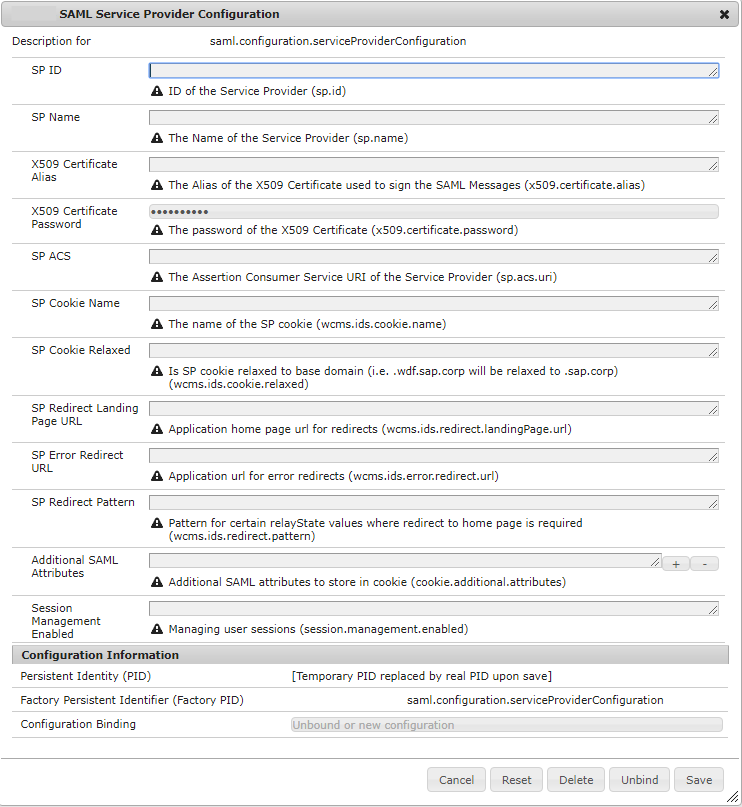
\includegraphics[width=\textwidth]{inc/svg/provider}
  \caption{Конфигурация поставщика сервиса}
  \label{fig:runConfig}
\end{figure}

\paragraph{Конфигурация поставщика учетных записей}

\begin{figure}[H]
  \centering
  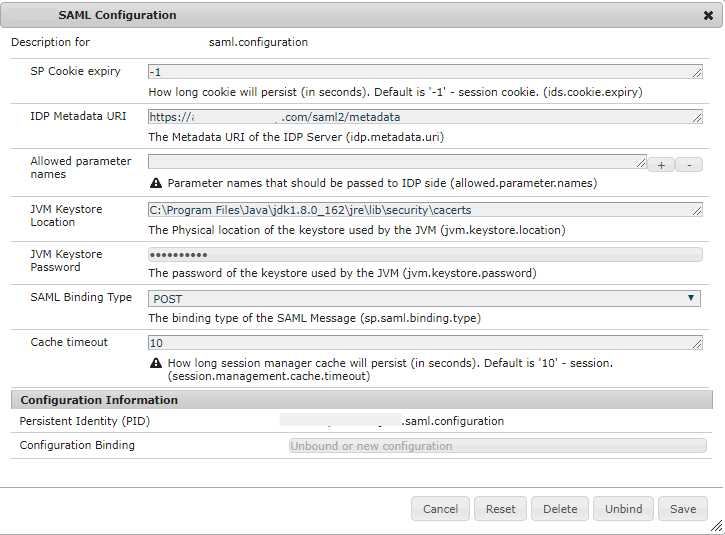
\includegraphics[width=\textwidth]{inc/svg/saml-config}
  \caption{Конфигурация поставщика учетных записей}
  \label{fig:samlConfig}
\end{figure}

%%% Local Variables:
%%% mode: latex
%%% TeX-master: "rpz"
%%% End:

